\chapter{Code Structure}
\label{cha:structure}
\section{Structure}
Our solution has been developed including 3 projects, 1 Core PCL project containing the application logic and 2 Platform implementation (Android and iOS) containing the specific platform code. 
The majority of the functionalities and the classes are placed in the PCL project, sharing the business logic across the implementation and leaving the customizations to the other projects. \\
In our PCL we can find the AppCore folder and the Framework folder, which contains respectively the implementation of the core logic and the abstract classes or interfaces that are implemented by the PCL itself or the platform projects.
Having used the MVVM architectural pattern in a Xamarin.Forms solution we tried to maximize the code sharing implementing as many functionalities in the ViewModel of the PCL project as well as realizing the UI (or Pages) of the application on the same project.
In this way, we use as many common UI components and features as possible, maximizing the code shared and using the platform code through the Dependency Service offered by Xamarin.Forms.
In the platform projects, there are the Dependencies folders that contain the platform implementations of the platform functionality needed to be shared. An example could be the implementation of the Toast notification, natively present in Android and customly implemented on iOS in the classes MessageImpl.
The Renderers, on the other hand, implements a native UI element changing the normal view of the Xamarin.Form element in something specifically customized for the platform.

\begin{figure}
	\centering
	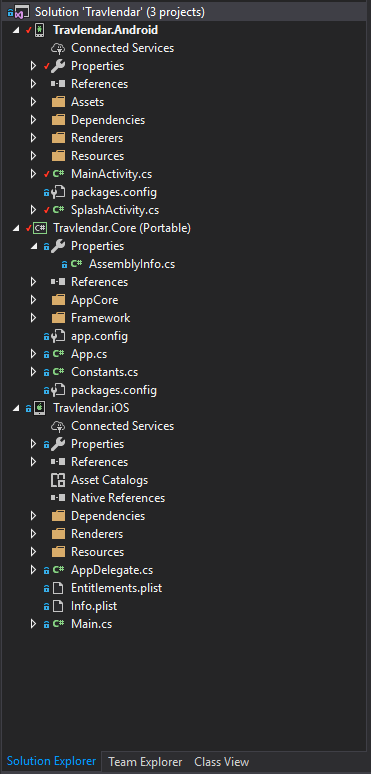
\includegraphics[width=4in]{./images/code_structure.png}
	\caption{Code Structure.}
	\label{fig:structure}
\end{figure}
